\documentclass[landscape,final,paperwidth=120cm,paperheight=90cm,fontscale=0.285]{baposter}%a0paper

\usepackage{calc}
\usepackage{graphicx}
\usepackage{amsmath}
\usepackage{amssymb}
\usepackage{relsize}
\usepackage{multirow}
\usepackage{rotating}
\usepackage{bm}
\usepackage{url}

\usepackage{graphicx}
\usepackage{multicol}

%\usepackage{times}
%\usepackage{helvet}
%\usepackage{bookman}
\usepackage{palatino}

\newcommand{\captionfont}{\footnotesize}

\graphicspath{{images/}{../images/}}
\usetikzlibrary{calc}

\newcommand{\SET}[1]  {\ensuremath{\mathcal{#1}}}
\newcommand{\MAT}[1]  {\ensuremath{\boldsymbol{#1}}}
\newcommand{\VEC}[1]  {\ensuremath{\boldsymbol{#1}}}
\newcommand{\Video}{\SET{V}}
\newcommand{\video}{\VEC{f}}
\newcommand{\track}{x}
\newcommand{\Track}{\SET T}
\newcommand{\LMs}{\SET L}
\newcommand{\lm}{l}
\newcommand{\PosE}{\SET P}
\newcommand{\posE}{\VEC p}
\newcommand{\negE}{\VEC n}
\newcommand{\NegE}{\SET N}
\newcommand{\Occluded}{\SET O}
\newcommand{\occluded}{o}
\newcommand{\argmax}{\operatornamewithlimits{argmax}}
\newcommand{\argmin}{\operatornamewithlimits{argmin}}

\newtheorem{asm}{Assumption}
\newtheorem{definition}{Definition}
\newtheorem{lemma}{Lemma}
\newtheorem{problem}{Problem}
\newtheorem{solution}{Solution}
\newtheorem{theorem}{Theorem}
\newtheorem{corollary}{Corollary}

%%%%%%%%%%%%%%%%%%%%%%%%%%%%%%%%%%%%%%%%%%%%%%%%%%%%%%%%%%%%%%%%%%%%%%%%%%%%%%%%
%%%% Some math symbols used in the text
%%%%%%%%%%%%%%%%%%%%%%%%%%%%%%%%%%%%%%%%%%%%%%%%%%%%%%%%%%%%%%%%%%%%%%%%%%%%%%%%

%%%%%%%%%%%%%%%%%%%%%%%%%%%%%%%%%%%%%%%%%%%%%%%%%%%%%%%%%%%%%%%%%%%%%%%%%%%%%%%%
% Multicol Settings
%%%%%%%%%%%%%%%%%%%%%%%%%%%%%%%%%%%%%%%%%%%%%%%%%%%%%%%%%%%%%%%%%%%%%%%%%%%%%%%%
\setlength{\columnsep}{1.5em}
\setlength{\columnseprule}{0mm}

%%%%%%%%%%%%%%%%%%%%%%%%%%%%%%%%%%%%%%%%%%%%%%%%%%%%%%%%%%%%%%%%%%%%%%%%%%%%%%%%
% Save space in lists. Use this after the opening of the list
%%%%%%%%%%%%%%%%%%%%%%%%%%%%%%%%%%%%%%%%%%%%%%%%%%%%%%%%%%%%%%%%%%%%%%%%%%%%%%%%
\newcommand{\compresslist}{%
\setlength{\itemsep}{1pt}%
\setlength{\parskip}{0pt}%
\setlength{\parsep}{0pt}%
}

%%%%%%%%%%%%%%%%%%%%%%%%%%%%%%%%%%%%%%%%%%%%%%%%%%%%%%%%%%%%%%%%%%%%%%%%%%%%%%
%%% Begin of Document
%%%%%%%%%%%%%%%%%%%%%%%%%%%%%%%%%%%%%%%%%%%%%%%%%%%%%%%%%%%%%%%%%%%%%%%%%%%%%%

\begin{document}

%%%%%%%%%%%%%%%%%%%%%%%%%%%%%%%%%%%%%%%%%%%%%%%%%%%%%%%%%%%%%%%%%%%%%%%%%%%%%%
%%% Here starts the poster
%%%---------------------------------------------------------------------------
%%% Format it to your taste with the options
%%%%%%%%%%%%%%%%%%%%%%%%%%%%%%%%%%%%%%%%%%%%%%%%%%%%%%%%%%%%%%%%%%%%%%%%%%%%%%
% Define some colors

%\definecolor{lightblue}{cmyk}{0.83,0.24,0,0.12}
\definecolor{lightblue}{rgb}{0.145,0.6666,1}

% Draw a video
\newlength{\FSZ}
\newcommand{\drawvideo}[3]{% [0 0.25 0.5 0.75 1 1.25 1.5]
   \noindent\pgfmathsetlength{\FSZ}{\linewidth/#2}
   \begin{tikzpicture}[outer sep=0pt,inner sep=0pt,x=\FSZ,y=\FSZ]
   \draw[color=lightblue!50!black] (0,0) node[outer sep=0pt,inner sep=0pt,text width=\linewidth,minimum height=0] (video) {\noindent#3};
   \path [fill=lightblue!50!black,line width=0pt] 
     (video.north west) rectangle ([yshift=\FSZ] video.north east) 
    \foreach \x in {1,2,...,#2} {
      {[rounded corners=0.6] ($(video.north west)+(-0.7,0.8)+(\x,0)$) rectangle +(0.4,-0.6)}
    }
;
   \path [fill=lightblue!50!black,line width=0pt] 
     ([yshift=-1\FSZ] video.south west) rectangle (video.south east) 
    \foreach \x in {1,2,...,#2} {
      {[rounded corners=0.6] ($(video.south west)+(-0.7,-0.2)+(\x,0)$) rectangle +(0.4,-0.6)}
    }
;
   \foreach \x in {1,...,#1} {
     \draw[color=lightblue!50!black] ([xshift=\x\linewidth/#1] video.north west) -- ([xshift=\x\linewidth/#1] video.south west);
   }
   \foreach \x in {0,#1} {
     \draw[color=lightblue!50!black] ([xshift=\x\linewidth/#1,yshift=1\FSZ] video.north west) -- ([xshift=\x\linewidth/#1,yshift=-1\FSZ] video.south west);
   }
   \end{tikzpicture}
}

\hyphenation{resolution occlusions}
%%
\begin{poster}%
  % Poster Options
  {
  % Show grid to help with alignment
  grid=false,
  % Column spacing
  colspacing=1em,
  % Color style
  bgColorOne=white,
  bgColorTwo=white,
  borderColor=lightblue,
  headerColorOne=black,
  headerColorTwo=lightblue,
  headerFontColor=white,
  boxColorOne=white,
  boxColorTwo=lightblue,
  % Format of textbox
  textborder=roundedleft,
  % Format of text header
  eyecatcher=true,
  headerborder=closed,
  headerheight=0.1\textheight,
%  textfont=\sc, An example of changing the text font
  headershape=roundedright,
  headershade=shadelr,
  headerfont=\Large\bf\textsc, %Sans Serif
  textfont={\setlength{\parindent}{1.5em}},
  boxshade=plain,
%  background=shade-tb,
  background=plain,
  linewidth=2pt
  }
  % Eye Catcher
  {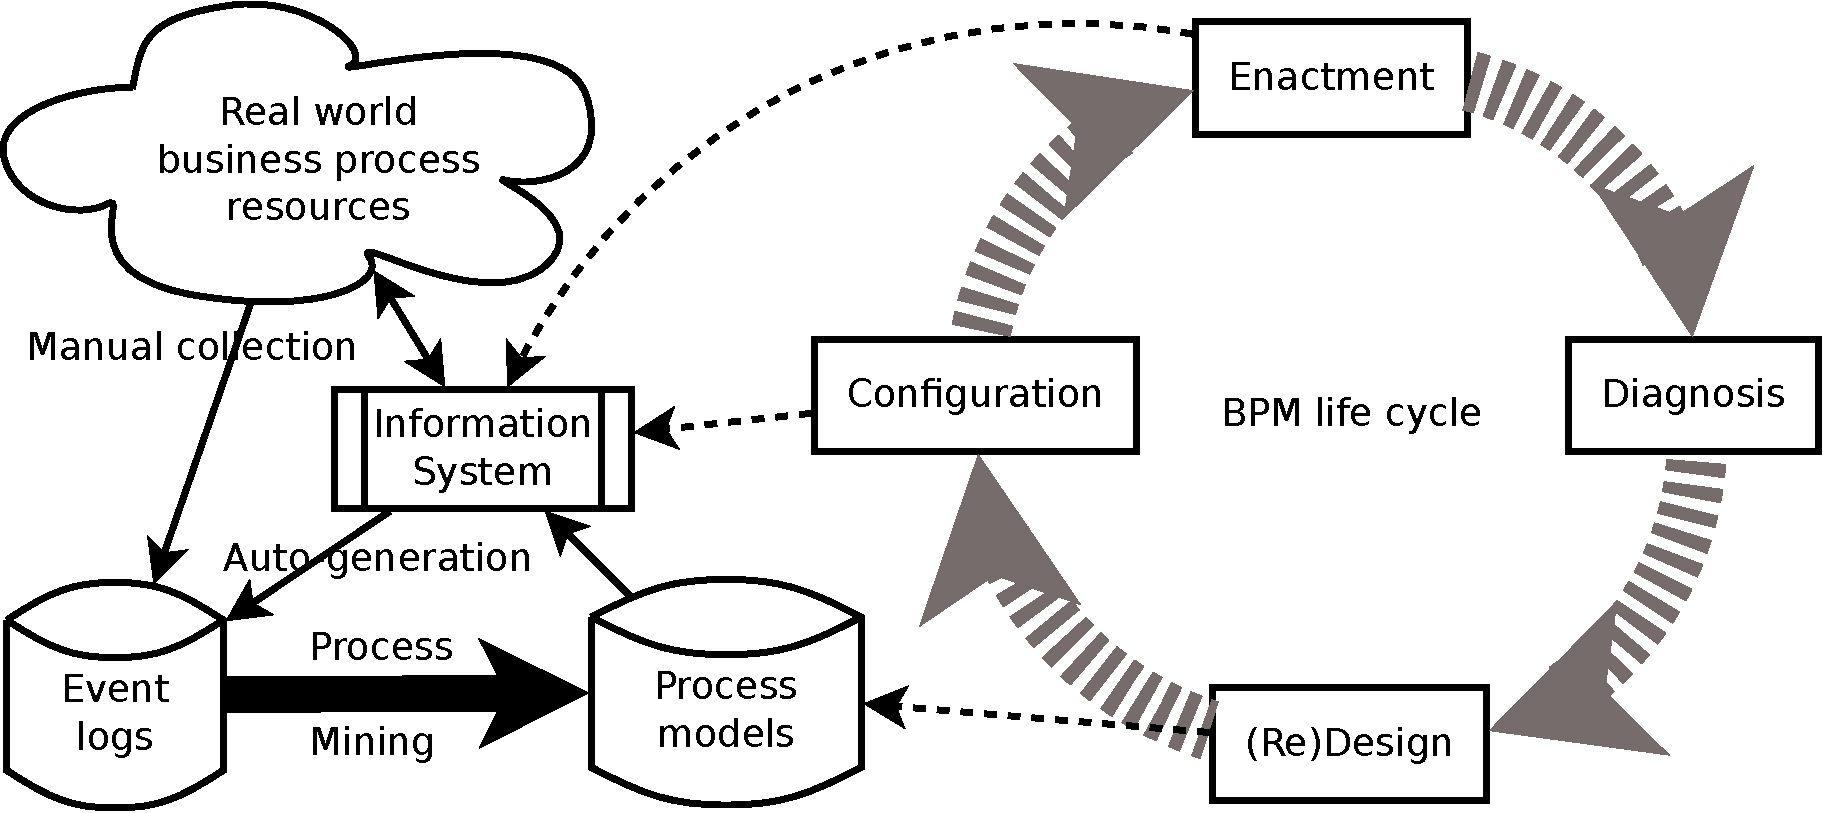
\includegraphics[height=5em]{images/bpmlifecycle.pdf}} 
  % Title
  {\bf\textsc{An Approach to Evaluate the Local Completeness of an Event Log}\vspace{0.5em}}
  % Authors
  {\textsc{Hedong Yang, Lijie Wen and Jianmin Wang\quad
		  School of Software, Tsinghua University}}
  % University logo
  {% The makebox allows the title to flow into the logo, this is a hack because of the L shaped logo.
    
\includegraphics[height=7.0em]{images/logo}
  }

%%%%%%%%%%%%%%%%%%%%%%%%%%%%%%%%%%%%%%%%%%%%%%%%%%%%%%%%%%%%%%%%%%%%%%%%%%%%%%
%%% Now define the boxes that make up the poster
%%%---------------------------------------------------------------------------
%%% Each box has a name and can be placed absolutely or relatively.
%%% The only inconvenience is that you can only specify a relative position 
%%% towards an already declared box. So if you have a box attached to the 
%%% bottom, one to the top and a third one which should be in between, you 
%%% have to specify the top and bottom boxes before you specify the middle 
%%% box.
%%%%%%%%%%%%%%%%%%%%%%%%%%%%%%%%%%%%%%%%%%%%%%%%%%%%%%%%%%%%%%%%%%%%%%%%%%%%%%
    %
    % A coloured circle useful as a bullet with an adjustably strong filling
    \newcommand{\colouredcircle}{%
      \tikz{\useasboundingbox (-0.2em,-0.32em) rectangle(0.2em,0.32em); \draw[draw=black,fill=lightblue,line width=0.03em] (0,0) circle(0.18em);}}
%%%%%%%%%%%%%%%%%%%%%%%%%%%%%%%%%%%%%%%%%%%%%%%%%%%%%%%%%%%%%%%%%%%%%%%%%%%%%%
  \headerbox{Background}{name=method,column=0}{
%%%%%%%%%%%%%%%%%%%%%%%%%%%%%%%%%%%%%%%%%%%%%%%%%%%%%%%%%%%%%%%%%%%%%%%%%%%%%%
  \noindent{\centering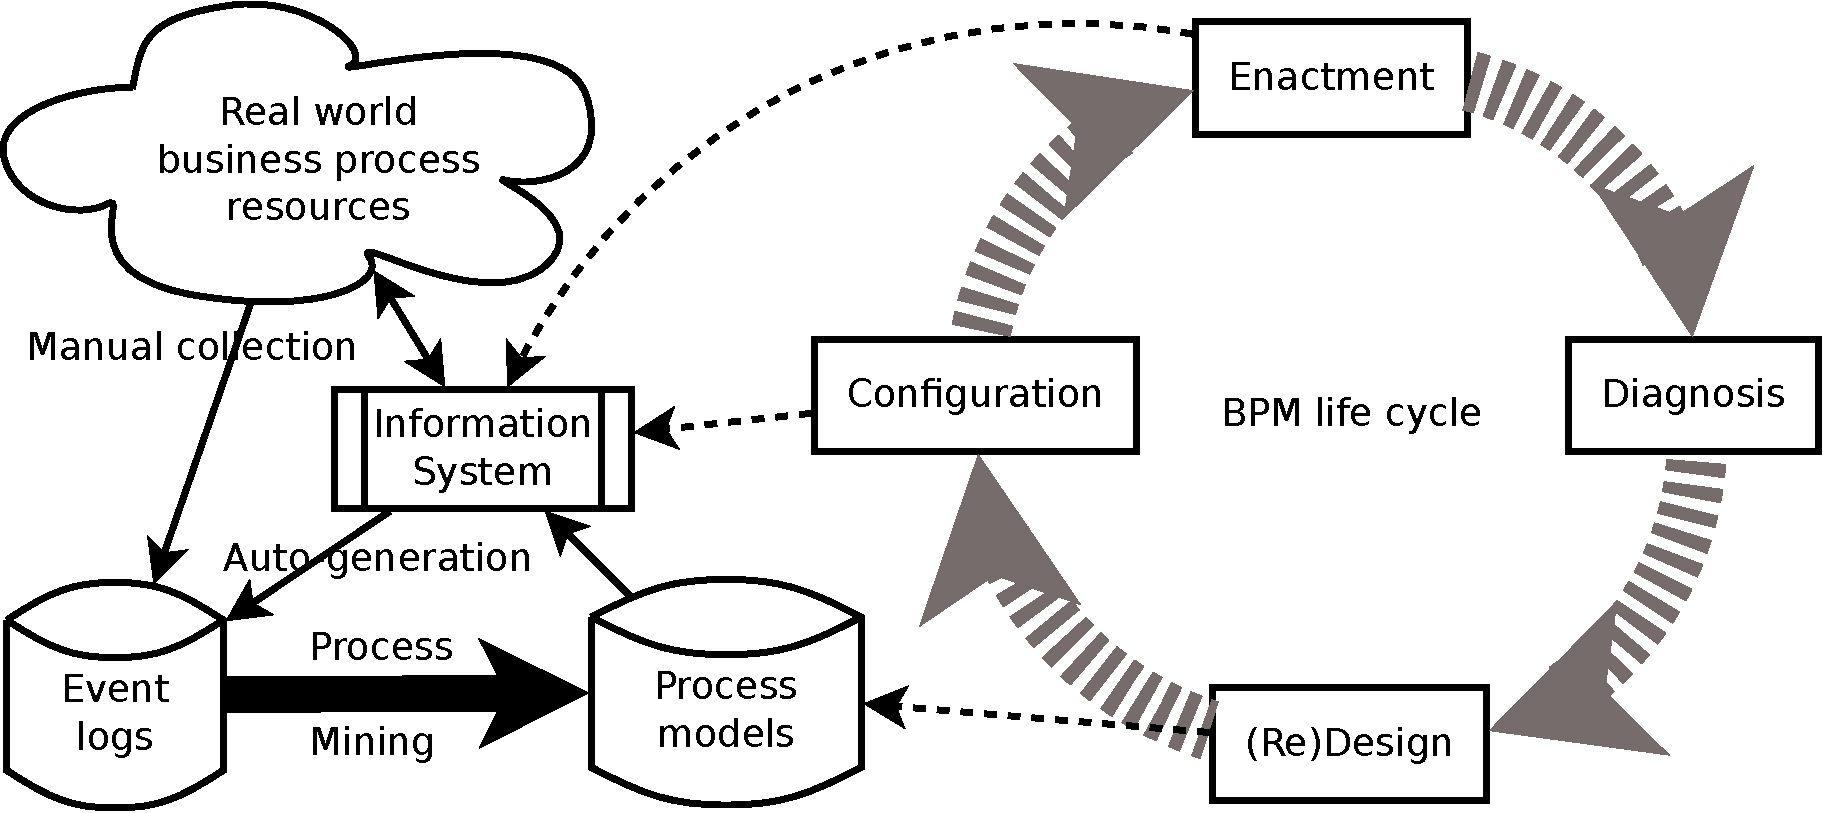
\includegraphics[width=0.95\linewidth]{images/bpmlifecycle.pdf}\\}
  \indent By means of deriving knowledge from event logs, process mining, which behaves 
  like the traditional data mining, is generally seen as a critical tool to
  improve operational business processes as well as concerned resources.
  Some mining algorithms assume the log to be \emph{locally complete}, i.e. all direct succession 
  (DS) relations between tasks of the underline process model should have been recorded in the given log.

  It is necessarily important to evaluate the local completeness of a log.
  However it is challenging because the process model is \emph{unknown}, based on which the local completeness
  is formulated.
   \vspace{0.3em}
  }
%%%%%%%%%%%%%%%%%%%%%%%%%%%%%%%%%%%%%%%%%%%%%%%%%%%%%%%%%%%%%%%%%%%%%%%%%%%%%%
  \headerbox{Characteristics of a Log}{name=background,column=1,bottomaligned=method}{
%%%%%%%%%%%%%%%%%%%%%%%%%%%%%%%%%%%%%%%%%%%%%%%%%%%%%%%%%%%%%%%%%%%%%%%%%%%%%%
%\noindent\begin{tabular}{r@{\hspace{0.3em}}c@{\hspace{1.5em}}c@{}}
%& With & Without\\
%& background model & background model\\
%\begin{sideways}{\makebox[0.37\linewidth][c]{Ridge of the lips}}\end{sideways} &
%\includegraphics[width=0.40\linewidth]{candidates_lips_ridge_left_bg} &
%\includegraphics[width=0.40\linewidth]{candidates_lips_ridge_left_no_bg} \\[2em]
%\end{tabular}
  \noindent 
\begin{asm}\label{asm:finite}
The total number of all possible tasks of process model is unknown but finite.
\end{asm}
\begin{asm}\label{asm:random}
A trace appears randomly and independently with its own probability which is
unknown.% constant value.
\end{asm}
\begin{asm}\label{asm:finite}
The given log is noise-free.
\end{asm}
%\iffalse
%\begin{table}%[!h] 
%	\begin{center}
%	\caption{The occurrence probabilities and frequencies of trace classes} 
%\begin{center}The occurrence probabilities and frequencies of trace classes\end{center} 
%	\label{tbl:tracefreqprob} 
	\begin{tabular}{lcccccc} 
		\hline%\noalign{\smallskip} 
		Trace classe&$T_1$ & $T_2$& $\cdots$ & $T_M$ & $\cdots$ & $T_W$\\ 
%		\noalign{\smallskip} \hline \noalign{\smallskip}
		Probability  &$p_1$ & $p_2$& $\cdots$ &  $p_M$ &  $\cdots$ & $p_W$\\ 
%		\noalign{\smallskip} \hline \noalign{\smallskip}
		Frequency&$\frac{\mu_1}{N}$&$\frac{\mu_2}{N}$&$\cdots$&$\frac{\mu_M}{N}$&$\cdots$&0\\
		\hline 
	\end{tabular} 
%	\end{center} 
%\end{table}
%\fi
%\caption{The occurrence probabilities and frequencies of DS relations}

%\begin{lemma}\label{thm:dsindependent}
\begin{equation*}
	\text{\textbf{Lemma:~~}}p_{x,y}=\sum_{i=1}^WS_{x,y}(i)Prob(T=t_i)
\end{equation*}
%\end{lemma}

\noindent{
\begin{tabular}{lcccccc}
\hline%\noalign{\smallskip}
DS &$T_1$ &  $\cdots$ & $T_W$& Prob. &Freq.\\
%\noalign{\smallskip} \hline \noalign{\smallskip}
$R_{1,1}$&$S_{1,1}(1)$&$\cdots$&$S_{1,1}(w)$&$p_{1,1}$&$\frac{\nu_{1,1}}{N}$\\
%\noalign{\smallskip} \hline \noalign{\smallskip}
%$R_{1,2}$&$S(2,1)$&$\cdots$&$S(2,W)$&$p_{1,2}$&$\frac{\nu_{1,2}}{N}$\\
%\noalign{\smallskip} \hline \noalign{\smallskip}
$\vdots$&$\vdots$&$\cdots$&$\vdots$&$\vdots$&$\vdots$\\
%\noalign{\smallskip} \hline \noalign{\smallskip}
$R_{r,r}$&$S_{r,r}(1)$&$\cdots$&$S_{r,r}(w)$&$p_{r,r}$&$\frac{\nu_{r,r}}{N}$\\
\hline
\end{tabular}
}
   \vspace{0.3em}
}


%%%%%%%%%%%%%%%%%%%%%%%%%%%%%%%%%%%%%%%%%%%%%%%%%%%%%%%%%%%%%%%%%%%%%%%%%%%%%%
\headerbox{Experiment Design}{name=speed,column=2,span=2,row=0}{
  %%%%%%%%%%%%%%%%%%%%%%%%%%%%%%%%%%%%%%%%%%%%%%%%%%%%%%%%%%%%%%%%%%%%%%%%%%%%%%
    \begin{multicols}{2}
		\noindent{\begin{center}Approaches to be compared\end{center}}
\begin{itemize}
%	\item Variants of our approach $CPL$
%	\begin{itemize}
	\item[-] \textbf{CPL.01} where $\varepsilon=0.01$,
	\item[-] \textbf{CPL.unit} where $\varepsilon=1/N$, 
	\item[-] \textbf{CPL.max} where $\varepsilon=\nu_{max}/N$,
	\item[-] \textbf{CPL.min} where $\varepsilon=\nu_{min}/N$,
	\item[-] \textbf{CPL.avg} where $\varepsilon=|\mathcal{S}|/N$.
%	\end{itemize}
%	\item Variants of the approach proposed in~\cite{vanhee:local}
%	\begin{itemize}
	\item [-] \textbf{KZN1} and \textbf{KZN2} (proposed in~\cite{vanhee:local})
	\item [-] \textbf{GCPL} (proposed in~\cite{hedong:global})
%	\end{itemize}
\end{itemize}

\noindent{\begin{center} Generated Logs for the experiments\end{center}}
\noindent{\begin{tabular}{lccccc}
\hline
Log type&Traces&DSes&Obsrv.&CompLen.\\%&Lower bound 1&Lower bound 2\\
\hline
Uniform &500&1001&1001&2654\\%&2524&2654\\
Normal &500&1001&1001&4790\\%&4441&4790\\
Pareto &500&1001&1000.4&\\
Long tail &1611&3223&3076&\\
\hline
\end{tabular}
}
\indent{} Each type contains 50 logs, and each log contains 10000 traces
randomly sampled.

\noindent{\begin{center}Open-accessed logs for the experiments\end{center}}
\indent{} 5  from the ProM web site contain 5 traces each.
\end{multicols}
   \vspace{0.0em}
  }

%%%%%%%%%%%%%%%%%%%%%%%%%%%%%%%%%%%%%%%%%%%%%%%%%%%%%%%%%%%%%%%%%%%%%%%%%%%%%%
  \headerbox{References}{name=references,column=0,above=bottom}{
%%%%%%%%%%%%%%%%%%%%%%%%%%%%%%%%%%%%%%%%%%%%%%%%%%%%%%%%%%%%%%%%%%%%%%%%%%%%%%
    \smaller
    \bibliographystyle{ieee}
    \renewcommand{\section}[2]{\vskip 0.05em}
      \begin{thebibliography}{1}\itemsep=-0.01em
      \setlength{\baselineskip}{0.4em}
%      \bibitem{hedong:local}
%        H.~Yang, L. Wen and J. Wang.
%        \newblock {An Approach to Evaluate the Local Completeness of an
%		Event Log}
%        \newblock In {\em ICDM '12}
      \bibitem{hedong:global}
        H. Yang, A. H. M. ter Hofstede, B. F. van Dongen, M. T. Wynn, and J. Wang.
        \newblock {On Global Completeness of Event Logs}
        \newblock In {\em BPMcenter.org '10}
      \bibitem{vanhee:local}
		K. M. van Hee, Z. Liu, and N. Sidorova.
        \newblock Is My Event Log Complete? - A Probabilistic Approach to Process Mining
        \newblock In {\em RCIS '11}
      \end{thebibliography}
   \vspace{0.3em}
  }
%%%%%%%%%%%%%%%%%%%%%%%%%%%%%%%%%%%%%%%%%%%%%%%%%%%%%%%%%%%%%%%%%%%%%%%%%%%%%%
\headerbox{Experiment Results}{name=results,column=2,span=2,row=0,below=speed,above=references}{
  %%%%%%%%%%%%%%%%%%%%%%%%%%%%%%%%%%%%%%%%%%%%%%%%%%%%%%%%%%%%%%%%%%%%%%%%%%%%%%
%    \drawvideo{2}{50}{%
%        \includegraphics[width=0.5\linewidth]{LengthF}%

\noindent{\begin{center}\textbf{Log Length Estimation on Generated Logs} \\
%		\includegraphics[width=0.25\linewidth]{images/LengthF}%
%        \includegraphics[width=0.25\linewidth]{images/LengthN}%
%        \includegraphics[width=0.25\linewidth]{images/LengthP}%
%        \includegraphics[width=0.25\linewidth]{images/LengthX}%
%\\
%    }
  \begin{tabular*}{\linewidth}{*{4}{@{}p{0.25\linewidth}@{}}}
 {\hfill{}Uniform logs\hfill{}} &{\hfill{}Normal logs\hfill{}} &
 {\hfill{}Pareto logs\hfill{}}  &{\hfill{}Long tail logs\hfill{}} 
  \end{tabular*}
% \\[1em]
  \end{center}}
      \vspace{-0.6em}
% \\[1em]

%     \drawvideo{5}{40}{%
%       \includegraphics[width=0.25\linewidth]{LengthX}%
%    }
% \begin{tabular*}{\linewidth}{*{5}{@{}p{0.2\linewidth}@{}}}
%   {\hfill{}Frame 0\hfill{}}  &
%   {\hfill{}100\hfill{}} &
%   {\hfill{}200\hfill{}} &
%   {\hfill{}300\hfill{}} &
%   {\hfill{}458\hfill{}} 
% \end{tabular*}
  \noindent{\begin{center}\textsc{\textbf{Conclusions}} \end{center}}
      \vspace{-0.6em}
     \begin{multicols}{2}
      \vspace{-0.6em}
\begin{itemize}
	\item CPL.max, CPL.01, and CPL.avg over-estimate on all kinds of logs,
	\item Both KZN1 and KZN2 do not work steadily,
	\item CPL.unit under-estimates on logs, and
	\item \textbf{\color{red}CPL.min performs the best} and robustly. Its results converge to the real lower bound of log length
on complete logs.%, and are closer to the real log length than any result from other approach on incomplete logs. %
\item GCPL under-estimates complete logs.
\end{itemize}
\end{multicols}
      \vspace{-0.6em}
%\caption[Lower bounds of completeness of example logs]{} \label{tbl:info}
\noindent{\begin{center}\textbf{Completeness Estimation on Public Logs:
		CPL.min vs. (GCPL)} 
\begin{tabular}{ccccccc}
\hline
Log & Length&$K=0.95$&$K=0.90$&$K=0.85$&$K=0.80$\\
\hline
a12f0n00\_1.xml&200 &97.78\%(n/a)    &98.43\%(n/a)    &98.72\%( 8.71\%)&98.89\%(20.94\%)\\
a12f0n00\_2.xml&600 &99.26\%( 8.71\%)&99.47\%(35.45\%)&99.57\%(47.30\%)&99.63\%(54.36\%)\\
a12f0n00\_3.xml&1000&99.55\%(29.29\%)&99.68\%(50.00\%)&99.74\%(59.18\%)&99.78\%(64.64\%)\\
a12f0n00\_4.xml&1400&99.68\%(40.24\%)&99.77\%(57.74\%)&99.82\%(65.50\%)&99.84\%(70.12\%)\\
a12f0n00\_5.xml&1800&99.75\%(47.30\%)&99.82\%(62.73\%)&99.86\%(69.57\%)&99.88\%(73.65\%)\\
\hline
\end{tabular}\end{center}}
      \vspace{-0.6em}
}

%%%%%%%%%%%%%%%%%%%%%%%%%%%%%%%%%%%%%%%%%%%%%%%%%%%%%%%%%%%%%%%%%%%%%%%%%%%%%%
  \headerbox{Formalized Problems}{name=problem,column=0,row=0,below=method,bottomaligned=results}{
%%%%%%%%%%%%%%%%%%%%%%%%%%%%%%%%%%%%%%%%%%%%%%%%%%%%%%%%%%%%%%%%%%%%%%%%%%%%%%
	The local completeness problem can formalized as the
	two following estimation problems:
      \vspace{1.6em}

	\noindent{}Given an event log $L$ of a process model $P$ (not known) and a confidence level $K$ ($0<K<1$),
\begin{problem}[Log length problem]\label{def:mathproblem}
 what should the minimal length $N$ of the
log be in order to be able to assert with confidence level $K$ that the
given log is locally complete, and 
\end{problem}
%
\begin{problem}[Local completeness problem]\label{def:problem}
how can we determine with confidence level $K$ what the ratio is
between the number of DS relations observed in $L$ versus the total number of
DS relations in all possible trace classes of $P$?
\end{problem}
   \vspace{0.3em}
 }

%%%%%%%%%%%%%%%%%%%%%%%%%%%%%%%%%%%%%%%%%%%%%%%%%%%%%%%%%%%%%%%%%%%%%%%%%%%%%%
  \headerbox{Solutions}{name=contribution,column=1,row=0,below=background,bottomaligned=results}{
%%%%%%%%%%%%%%%%%%%%%%%%%%%%%%%%%%%%%%%%%%%%%%%%%%%%%%%%%%%%%%%%%%%%%%%%%%%%%%
   \begin{theorem}\label{thm:dsinfo}
Let $N$ be the length of a log. It holds that 
$ P\left\{\varepsilon \geq G-p_v\right\} > 1 -
\frac{p_u(1-p_u)}{N\varepsilon^2}$,
where $1>\varepsilon>0$, $G=p_u+p_v$, $p_v$ and $p_u$ is the probabilities of DS relations
observed and unobserved respectively.
\end{theorem}
Given an event log $L$ of a process model $P$ (not known) and a confidence level $K$ ($0<K<1$), 
\begin{solution}the length $N$
of the log should be greater than $\frac{1}{\varepsilon\sqrt{1-K}}-1$ in
order to be able to assert with confidence level $K$ that the given log is
locally complete, 
\end{solution}
\begin{solution} and with confidence level $K$, the ratio of observed DS relations in $L$ versus those in
	$P$ is estimated by means of occurrence probability 
	to have an upper bound value of $1-\frac{1}{(N+1)\sqrt{1-K}}$.
\end{solution}
   \vspace{0.3em}
}

%%%%%%%%%%%%%%%%%%%%%%%%%%%%%%%%%%%%%%%%%%%%%%%%%%%%%%%%%%%%%%%%%%%%%%%%%%%%%%
  \headerbox{Future Directions}{name=questions,column=1,span=2,aligned=references,above=bottom}{
%%%%%%%%%%%%%%%%%%%%%%%%%%%%%%%%%%%%%%%%%%%%%%%%%%%%%%%%%%%%%%%%%%%%%%%%%%%%%%
  \begin{multicols}{2}
    The approach may be extended by considering both the number of appearances of a DS relation 
	and the co-appearances of DS relations in a trace, which are ignored in
	the current approach.
    
	Since the assumptions that underpin our approach are similar to those for solutions to
	the global completeness problem, the approach may be extended for the global completeness problem.
  \end{multicols}
   \vspace{0.3em}
  }
%%%%%%%%%%%%%%%%%%%%%%%%%%%%%%%%%%%%%%%%%%%%%%%%%%%%%%%%%%%%%%%%%%%%%%%%%%%%%%
  \headerbox{Source Code}{name=references,column=3,aligned=references,above=bottom}{
%%%%%%%%%%%%%%%%%%%%%%%%%%%%%%%%%%%%%%%%%%%%%%%%%%%%%%%%%%%%%%%%%%%%%%%%%%%%%%
  The source code of the approach as a plug-in of an evaluation framework is available at \\
  \url{https://github.com/hunter99/CompletenessFramework}
   \vspace{0.3em}
  }
\end{poster}

\end{document}
